\documentclass{article}
\usepackage[utf8]{inputenc}
\usepackage[margin=1.0in]{geometry}
\usepackage{amsmath}
\usepackage{amssymb}
\usepackage{fancyhdr}
\usepackage{physics}
\usepackage{wrapfig}
\usepackage{hyperref}
\usepackage{multirow}
\usepackage{amsthm}
\usepackage{pgfplots}

\pgfplotsset{compat=1.16}



\renewcommand{\thesubsection}{\thesection\Alph{subsection}}
\renewcommand\qedsymbol{\square}



\title{Particle Physics PS1}
\author{Joe Crowley}
\date{October 2020}

\pagestyle{fancy}
\renewcommand{\headrulewidth}{0pt}
\renewcommand{\footrulewidth}{1pt}

\fancyhf{}
\rhead{
Joe Crowley \\
Physics 225 \\
Problem Set 2\\
}
\rfoot{Page \thepage}

\begin{document}  


\section{Questions on natural units}

\subsection{}
\textit{The cross section for the process $e^{+} e^{-} \rightarrow \mu^{+} \mu^{-}$ (via a virtual photon) is given by $\sigma=\frac{4 \pi}{3} \frac{\alpha^{2}}{E_{\mathrm{cm}}^{2}}$ in n.u., where $E_{\mathrm{cm}}$ is the total energy in the center-of-momentum frame. (This formula applies for $\left.E_{\mathrm{CM}}>>m_{\mu} .\right)$ What are the required dimensions of a cross section? Use this fact to restore any needed powers of $\hbar$ and $c$ to the cross section formula. Next, compute the numerical value of this cross section at $E_{\mathrm{CM}}=1 \mathrm{GeV}$ in the units of barns, where 1 barn $=1 \mathrm{b}=10^{-24} \mathrm{cm}^{2}$}

\begin{align*}
    [\sigma]&=[L]^{2}\\
    [L]^2 &= [E]^{-2}[E L ]^2\\
    \implies \sigma &= \frac{4 \pi}{3} \frac{\alpha^{2}}{E_{\mathrm{cm}}^{2}} (\hbar c)^2\\
    &= 8.68545 \times 10^{-36} \, \mathrm{m}^{2}\\
    &= 8.68545 \times 10^{-8} \,\mathrm{barns}
\end{align*}


\subsection{}
\textit{When a low energy photon scatters from an atomic electron, there is an energy regime in which $E_{B}<<E(\gamma)<<m_{e} .$ (Here $E_{B}$ is the atomic binding energy.) This is called Thomson scattering, and the cross section is given by
$$
\sigma\left(\gamma e^{-} \rightarrow \gamma e^{-}\right)=\frac{8 \pi}{3}\left(\frac{\alpha}{m_{e}}\right)^{2}
$$
Restore any needed powers of $\hbar$ and $c,$ and then evaluate the scattering cross section in $\mathrm{cm}^{2} .$ Hint: $\sigma=6.6 \times 10^{-25} \mathrm{cm}^{2}$}

\begin{align*}
    [\sigma]&=[L]^{2}\\
    [L]^2 &= [E]^{-2}[E L ]^2\\
    \implies \sigma\left(\gamma e^{-} \rightarrow \gamma e^{-}\right)&=\frac{8 \pi}{3}\left(\frac{\alpha}{m_{e} c^2 }\right)^{2}  (\hbar c)^2\\
    &= \frac{8 \pi}{3}\left(\frac{\alpha \hbar}{m_{e} c}\right)^{2}\\
    &=6.6 \times 10^{-29} \mathrm{m}^{2}\\
    &=6.6 \times 10^{-25} \mathrm{cm}^{2}
\end{align*}

\subsection{}
\textit{Bohr radius, Compton wavelength, and "classical" electron radius. Recall that, in n.u., the Bohr radius of the H-atom is $a_{0}=1 /\left(m_{e} \alpha\right)$ and the Compton wavelength of the electron is $\lambda_{C}=1 / m_{e} .$ From the discussion of Thomson scattering, you can see that we can define a length scale $r_{0}=$ $\alpha / m_{e}$ in which $\alpha$ is in the numerator. This quantity is called the classical electron radius. Make a table listing the values of these three quantities. We will later see that the Compton wavelength is extremely important, because it sets a length scale below which quantum field theory must be used rather than a single particle wave equation (for the given type of particle}

\begin{table}[]
    \centering
    \begin{tabular}{||c|c|c||}
        \hline\hline$a_{0}$ & $\lambda_{c}$ & $r_{0}$ \\
        \hline$\frac{1}{\alpha m_{e}}$ & $\frac{1}{m_{e}}$ & $\frac{\alpha}{m_{e}}$ \\
        \hline $0.529 \AA$ & $386 \mathrm{fm}$ & $2.82 \mathrm{fm}$ \\
        \hline\hline
    \end{tabular}
    \caption{Bohr radius, Compton wavelength, and "classical" electron radius.}
    \label{tab:my_label}
\end{table}




\newpage


\section{Simple relativity: Lorentz invariant quantities}
\textit{Consider two arbitrary four vectors, $a=\left(a^{0}, \vec{a}\right)$ and $b=\left(b^{0}, \vec{b}\right)$.}

\subsection{}
\textit{Show explicitly that the dot product
$$
a \cdot b=a^{0} b^{0}-\vec{a} \cdot \vec{b}
$$
is invariant under a Lorentz transformation along the $z$ axis. In other words show that $a^{\prime} \cdot b^{\prime}=a \cdot b,$ where $a^{\prime}$ and $b^{\prime}$ are the Lorentz-transformed four vectors.}
\begin{align*}
    a \cdot b&=a^{\prime} \cdot b^{\prime}\\
    (a^\prime)^{\mu} (b^\prime)_{\mu}&=\Lambda_{\;\rho}^{\mu} a^{\rho} \Lambda_{\mu}^{\;\sigma} b_{\sigma}\\
    &=\Lambda^{\mu} _{\;\rho} \Lambda_{\mu}^{\;\sigma} a^{\rho} b_{\sigma}\\
    &=\delta_{\rho}^{\sigma} a^{\rho} b_{\sigma} \\
    &= a^{\rho} b_{\rho} \\
    &= a \cdot b
\end{align*}

\begin{equation*}
    \boxed{ a \cdot b=a^{\prime} \cdot b^{\prime}}
\end{equation*}

\subsection{}
\textit{Suppose that two four-vectors are given by $a=(10.5,4.3,-5.6,7.9)$ (in some units) and $b=(-22.6,-3.5,6.6,50.4)$ (in some other units). Suppose that in another reference frame, $a^{\prime}=(7.777,4.3,-5.6,-3.556) .$ What are the parameters $\beta$ and $\beta \gamma$ for the Lorentz transformation? Compute $b^{\prime}$ and verify that $a \cdot a=a^{\prime} \cdot a^{\prime}$ and $a \cdot b=a^{\prime} \cdot b^{\prime}$}

The lorentz boost is along the z axis, because the x and y components of $a$ remain unchanged. Therefore, the equations for the primed variables are: 
\begin{align*}
t^{\prime}&=\gamma t-\beta \gamma z \\
z^{\prime}&=\gamma z-\beta \gamma t \\
\end{align*}

Solving these equations for $\gamma$ and $\beta\gamma$,

\begin{align*}
\gamma&=\frac{t t^{\prime}-z z^{\prime}}{t^{2}-z^{2}}=2.29412 \\
\beta \gamma&=\frac{z t^{\prime}-t z^{\prime}}{t^{2}-z^{2}}=2.06472
\end{align*}

Verifying the lorentz invariance of $a^2 = (a^\prime)^2$,

\begin{align*}
a \cdot &a=-2.01 \\
a^{\prime} \cdot a^{\prime}&=-2.013
\end{align*}

\begin{align*}
b \cdot b&=-2085.21 \\
b^{\prime} \cdot b^{\prime}&=-2085.07
\end{align*}


\subsection{}
\textit{Suppose a particle has four-momentum $p=(E, \vec{p})$ in some reference frame. What is the Lorentz transformation to the CM frame, where $\vec{p}^{\prime}=0 ?$ You may choose $\vec{p}$ to point in a particular direction for convenience. In the CM frame, what is the interpretation of $E ?$ Given this, what is the interpretation of $E^{2}-\vec{p}^{2}$ in an arbitrary reference frame?}

\begin{equation}
\left(\begin{array}{l}
m \\
0 \\
0 \\
0
\end{array}\right)=\left(\begin{array}{llll}
\gamma & 0 & 0 & -\beta \gamma \\
0 & 1 & 0 & 0 \\
0 & 0 & 1 & 0 \\
-\beta \gamma & 0 & 0 & \gamma
\end{array}\right)\left(\begin{array}{l}
E \\
0 \\
0 \\
p
\end{array}\right)
\end{equation}

\begin{align*}
\beta \gamma&=\frac{m p}{E^{2}-p^{2}} \\
\gamma&=\frac{E m}{E^{2}-p^{2}}
\end{align*}

in an abitrary reference frame, $m^{2}=E^{2}-\vec{p}^{2}$ is the lorentz invariant  mass squared.

\subsection{}
\textit{A particle has four-momentum $p=(4.0,0.0,0.0,2.5315) \mathrm{GeV} .$ What is the mass of a particle? What particle is this?}

\newpage


\section{Decay of a free photon?}
\textit{Using relativity, show that the process $\gamma \rightarrow e^{+} e^{-}$ cannot occur in the vacuum. Here the photon is a free particle, not a virtual photon. Your argument should be mathematical, not just verbal.}

\newpage


\section{}
\textit{Let $G$ be a group. Prove that}

\subsection{}
\textit{The identity element of $G$ is unique.}

\subsection{}
\textit{Every element $a \in G$ has a unique inverse in $G$.}

\newpage


\section{Kinematics of scattering in a fixed-target experiment.}
\textit{A beam of particles with mass $M_{A}$ and energy $E_{A}$ is incident on a target containing particles of mass $M_{B}$ at rest, resulting in the process $A+B \rightarrow$ $1+2+\ldots+N .$ The final-state particles have masses $m_{1}, m_{2}, \ldots, m_{N}$}
\subsection{}
\textit{True or false: $M_{A}+M_{B}=m_{1}+m_{2}+\ldots+m_{N} .$ If true, explain why. If not, give an alternative statement.}

\subsection{}
\textit{Compute the minimum value of the energy of particle $\mathrm{A}, E=E_{A}^{\min },$ for the process to be kinematically allowed.}

\subsection{}
\textit{Consider the case of a $\tau$ neutrino with energy $E_{\nu}$ that is incident on a neutron at rest. What is the minimum value of $E_{\nu}^{\min }$ for the neutrino to produce a $\tau$ -lepton via the process $\nu_{\tau}+n \rightarrow \tau^{-}+p ?$ (You may neglect the neutrino mass in the calculation. You may use $m_{p}=938 \mathrm{MeV}, m_{n}=940$ $\mathrm{MeV},$ and $\left.m_{\tau}=1777 \mathrm{MeV} .\right)$}

\newpage


\section{Colliding electron and positron beams at asymmetric energies.}
\textit{In the PEP-II storage ring at SLAC, the electron and positron beam energies were, respectively, $E_{1}=9.0 \mathrm{GeV}$ and $E_{2}=3.1 \mathrm{GeV} .$ The beams collided head on.}
\subsection{}
\textit{What is the total energy of the $e^{+} e^{-}$ system in the CM frame (the frame in which the total momentum is zero)?}

\subsection{}
\textit{What $\Upsilon$ (a $b \bar{b}$ system) state is closest to this energy? These mesons are created in very large quantities (hundreds of millions) at PEP-II. What is the dominant decay mode of this $\Upsilon$ state?}

\subsection{}
\textit{What are the velocity $\beta$ and the factor $\beta \gamma$ for the Lorentz transformation from the lab frame to the CM frame?}


\subsection{}
\textit{What are the beam energies in the CM frame?}


\subsection{}
\textit{Using the web, try to find a description or a photo of the inside of the PEP-II ring. How were the two beams stored in this accelerator? What did it look like inside the tunnel?}



\newpage


\section{Momenta in two body decay of a particle. }
\textit{In Lecture $4,$ we calculated the energies of the outgoing particles 1 and 2 in the decay $A \rightarrow 1+2 .$ For the record let's calculate the magnitudes of the corresponding momenta. Show that
$$
\left|\mathbf{p}_{1}\right|=\left|\mathbf{p}_{2}\right|=\frac{\lambda^{1 / 2}\left(m_{A}^{2}, m_{1}^{2}, m_{2}^{2}\right)}{2 m_{a}}
$$
where the function $\lambda$ is given by
$$
\lambda(x, y, z)=x^{2}+y^{2}+z^{2}-2 x y-2 x z-2 y z
$$}

\newpage


\section{}
\textit{Mandelstam variables. Consider a scattering process $1+2 \rightarrow 3+4,$ where the 4 -momenta of the particles are $p_{1}, p_{2}, p_{3},$ and $p_{4} .$ The Mandelstam variables are the Lorentz-invariant quantities
$$
\begin{aligned}
s &=\left(p_{1}+p_{2}\right)^{2} \\
t &=\left(p_{3}-p_{1}\right)^{2} \\
u &=\left(p_{1}-p_{4}\right)^{2}
\end{aligned}
$$
These variables provide an alternate way to specify the same information that is contained in the (Lorentz-invariant) inner products of the four momenta.}
\subsection{}
\textit{Show that
$$
s+t+u=m_{1}^{2}+m_{2}^{2}+m_{3}^{2}+m_{4}^{2}
$$}

\subsection{}
\textit{Compute $s, t,$ and $u$ in the CM frame in the relativistic limit $m_{i}=0$ Express the result in terms of the CM-frame scattering angle $\theta$ and the magnitude of the momentum of either particle in the CM frame, $\left|\vec{p}_{C M}\right|$. Compute $s+t+u$ for this case.}


\newpage


\section{Charged pion decay.}
\textit{(Based on Griffiths problem 3.15 ) A pion traveling at speed $v$ in the lab frame decays into a muon and a neutrino, $\pi^{-} \rightarrow \mu^{-} \bar{\nu}_{\mu}$}
\subsection{}
\textit{What is the branching fraction for this decay?}


\subsection{} 
\textit{What is the second most common $\pi^{-}$ decay?}

\subsection{} 
\textit{Neutrino beams are created by arranging for a beam of high-momentum charged pions to decay in a long beam pipe. What kind of neutrinos are mainly created in such beams?}

\subsection{} 
\textit{If the neutrino emerges at $90^{\circ}$ to the original pion direction, at what angle does the $\mu$ come off? Discuss the behavior of this result. Hint: $\tan \theta=$ $\left(1-m_{\mu}^{2} / m_{\pi}^{2}\right) /\left(2 \beta \gamma^{2}\right)$}


\begin{figure}[h!]
    \centering
    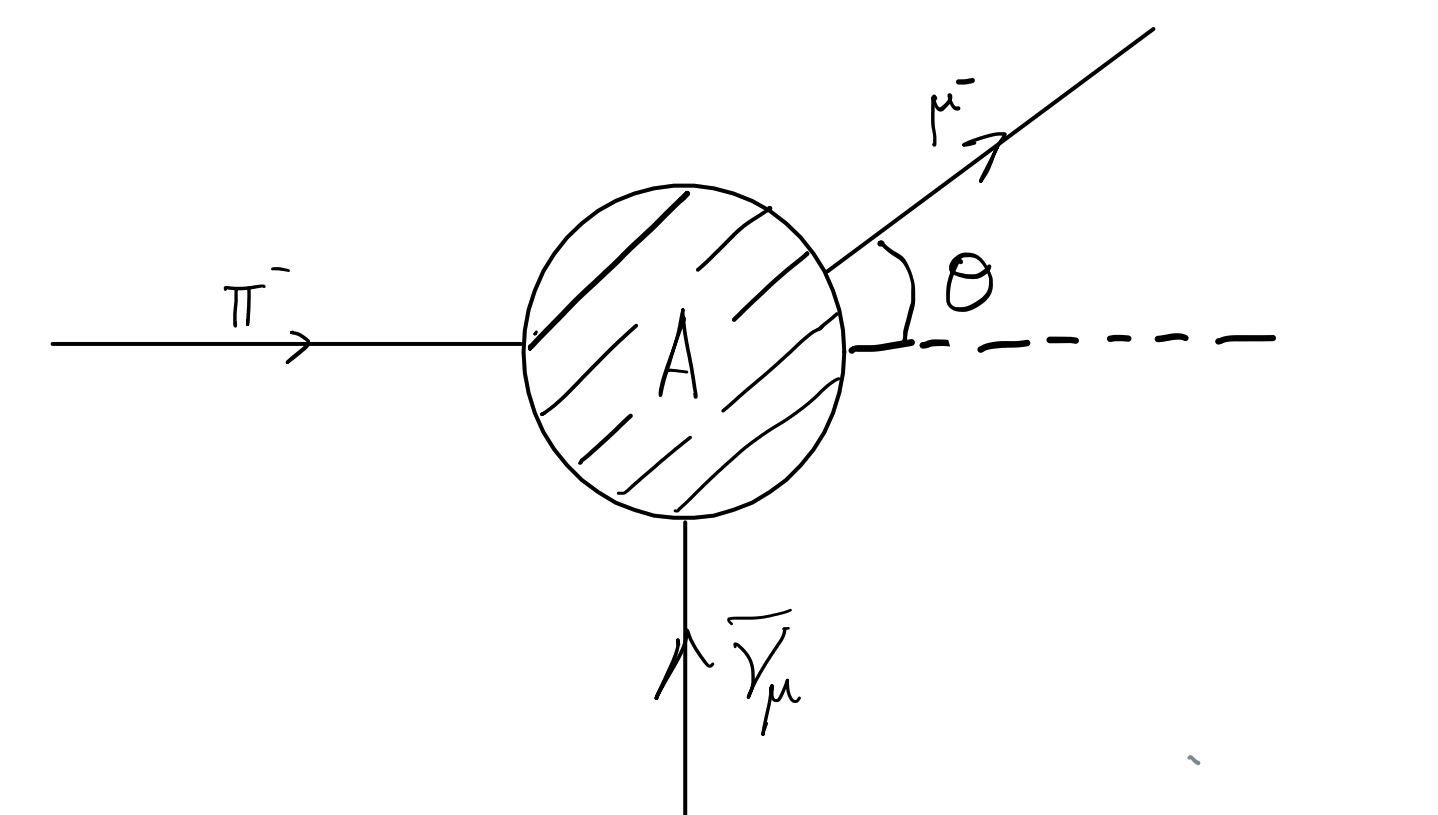
\includegraphics[width=0.5\textwidth]{figures/problem_9.png}
    \label{fig:my_label}
\end{figure}



\newpage


\section{The rapidity variable for hadron collider physics.}
\textit{In a hadron collider, the rapidity variable
$$
y=\frac{1}{2} \ln \frac{E+p_{z}}{E-p_{z}}
$$
is frequently used. Here $z$ is the beam direction.}


\subsection{}
\textit{Show that the difference $\Delta y$ in rapidity between two particles is invariant under Lorentz boosts along the $z$ direction. To do this, first show that under a Lorentz boost in the $z$ -direction the rapidity transforms as
$$
y^{\prime}=y+\frac{1}{2} \ln \frac{1-\beta}{1+\beta}
$$}


\subsection{}
\textit{Consider the case in which the mass of the particle (or, as is often the case, the jet) is ignored and take $p_{z} \approx E \cos \theta .$ Under this assumption show that $y$ can be approximated by the pseudorapidity
$$
\eta=-\ln \left(\tan \frac{\theta}{2}\right)
$$}d

\end{document}
